\section{Vertex-Centric Storage for Property Graph}\label{sec:storage}
%The random access problem is a well known hard problem for out-of-core systems, especially for the graph related problem, which is notorious for its poor locality~\cite{DBLP:conf/osdi/KyrolaBG12}.

Many graph computing frameworks store graphs on disk using the double list method:
storing the in-edges and out-edges \textbf{separately} for each vertex,
via the compressed sparse column (CSC) and the compressed sparse row (CSR) format~\cite{DBLP:conf/sc/PearceGA10}.
However, this separation incurs excessive random access on real-world property graph because we need to get the information for in/out edges during pattern matching.

Instead, SeqStar stores the graph data in a vertex-centric way which stores all the information related to one vertex \textbf{together}.
With small indexes on disks, pattern matching can quickly get the correct address of relevant data on disk during pattern matching. Because all the related information is stored together, SeqStar can make sure that all disk reads are sequential.

Moreover, by using the property graph matching engine that will be discussed in the next section,
the huge data graph will be read at most once.
\subsection{Scan the Data Graph Sequentially}
%The property graph matching problem requires the complete connection information between vertices,
%however, the conventional double list storage method break up the completeness and results in random disk accesses.

Consider the example in Figure~\ref{img:running_example}.
If two vertices in the data graph, say $v_i$ and $v_j$, are supposed to match $u_1$ and $u_2$,
we must be sure that $v_i$ and $v_j$ follows each other at the same time.
This kind of neighbor checking is the most essentially building block of a property graph matching engine.

In the data graph, vertex $1$ has $4$ in-edges and $7$ out-edges.
Suppose that they are stored separately in the traditional way.
In order to determine whether vertex $1$ could match $u_1$,
one has to scan the in-edges (or equally, the out-edges) of vertex $1$ and then check whether the visited neighbor is in the out-edges (or in-edges) list.
Such a scan and check method would significantly slow down the graph matching process,
because the checking process results in random disk reads.
For real world power-law graphs, where the celebrities or trending topics have a huge amount of followers, this phenomenon greatly exacerbate the random access problem.
%the in/out-edges lists stored on disk have to be swapped in and out frequently during the scan and check process as a result of the random disk access pattern.
%% Multiple edges between $u_1$ and $u_2$ make things even worse.
%And it would be more complicated if there are more than two edges between $u_1$ and $u_2$ in the pattern graph.

On the contrarily, SeqStor's vertex-centric storage keeps the necessary connection information together for graph matching.
Figure~\ref{img:data_example} shows the logical structure for the data graph in Figure~\ref{img:running_example}.
The specific edge information (direction, types) could be obtained by the stored edge labels, i.e., the top labels associate to the out-edges and the bottom labels associate to the in-edges (Figure~\ref{img:data_example}).

\begin{figure}[ht]
  \centering
  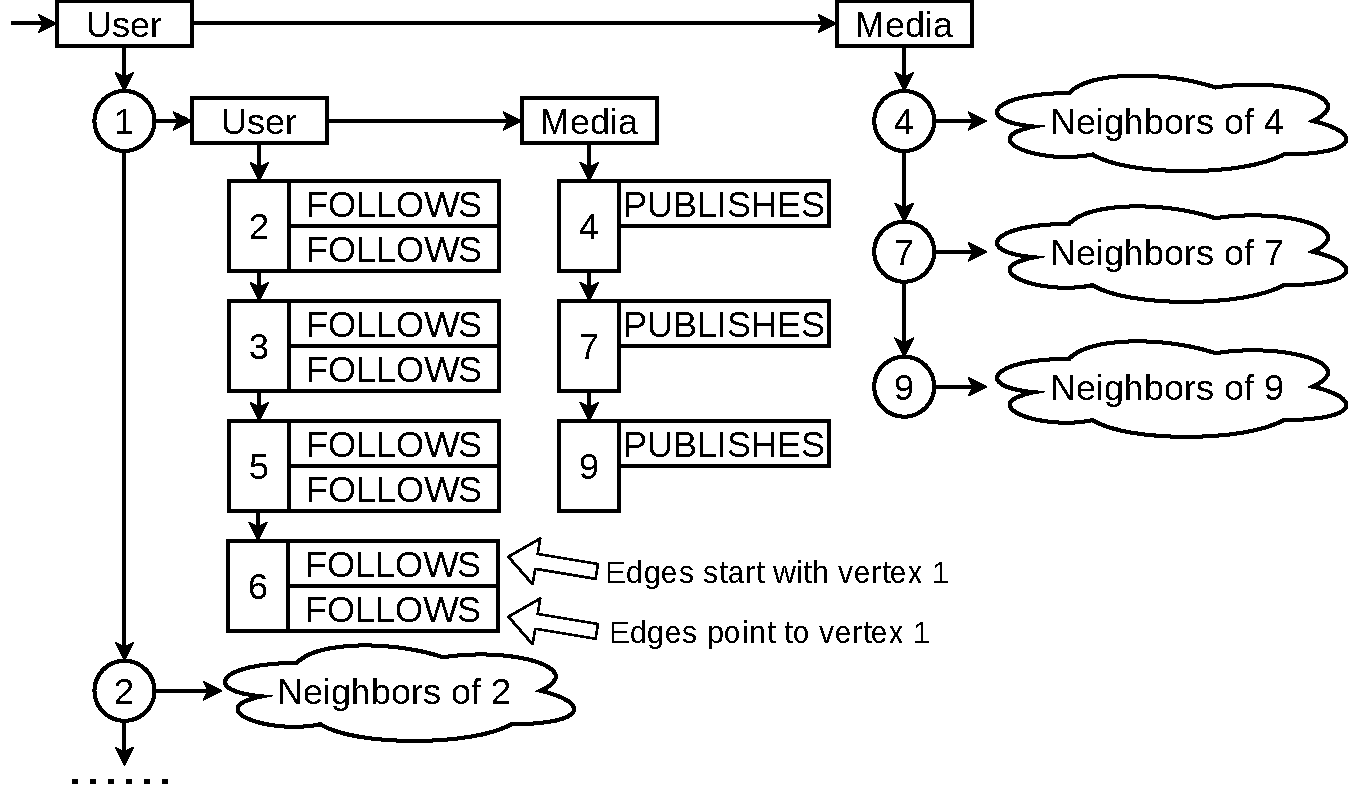
\includegraphics[width=0.5\textwidth]{img/data_example.pdf}
  \caption{Vertex-centric graph data storage.}\label{img:data_example}
\end{figure}

By using the vertex centric graph data storage, the neighborhood checking process can be accomplished efficiently within a sequential disk scan.
For $S_1$ in Figure~\ref{img:running_example},
to check the neighbors of vertex $1$, SeqStar scans the neighbors $2, 3, 5, 6$ and $4, 7, 9$ sequentially.
No random disk access appears during the whole process.
\subsection{Graph Data Indexes}
%Despite of the fact that the size of the whole data graph could be gigantic,we may only care a fraction of the graph by specify the labels in our query for a concrete graph matching problem.
There are two basic operations in a graph matching engine:
(1) Given a data vertex, retrieve its neighbors with a specific label;
(2) Given a vertex label, retrieve the vertices with the label.
%% In the following paragraphs, we'll show how to make the two operations efficiently by adding a few simple but efficient indices to the vertex-centric storage engine,
%% which reduces the searching space and I/O significantly.

Consider the data graph in Figure~\ref{img:running_example}.
One may want to study only the relationships among users.
For vertex $1$ in the figure,
no matter how much social media she has published or viewed we could just ignore all of them in this specific problem.
%% A straightforward idea is to group the neighbor vertices with the same label together when storing the vertices.
%% However, if the neighbor vertices were stored in the traditional in/out-edge double lists method,
%% we have to group them twice and then still face the information insufficient problem as we discussed in the previous subsection.
%% As for our vertex-centric storage method,
For SeqStor's vertex-centric storage method,
the index could be added to the storage engine easily as shown in Figure~\ref{img:data_example}.
These indexes are key-value pairs mapping the vertex labels to the starting/ending position of the neighbors on disk.
Since it is used to locate only the neighbors of a specific vertex, we refer to this kind of index as \emph{local index}.
With the help of local index, we could skip all the useless neighbor vertices and only scan the necessary ones.
%% \begin{figure}[ht]
%%   \centering
%%   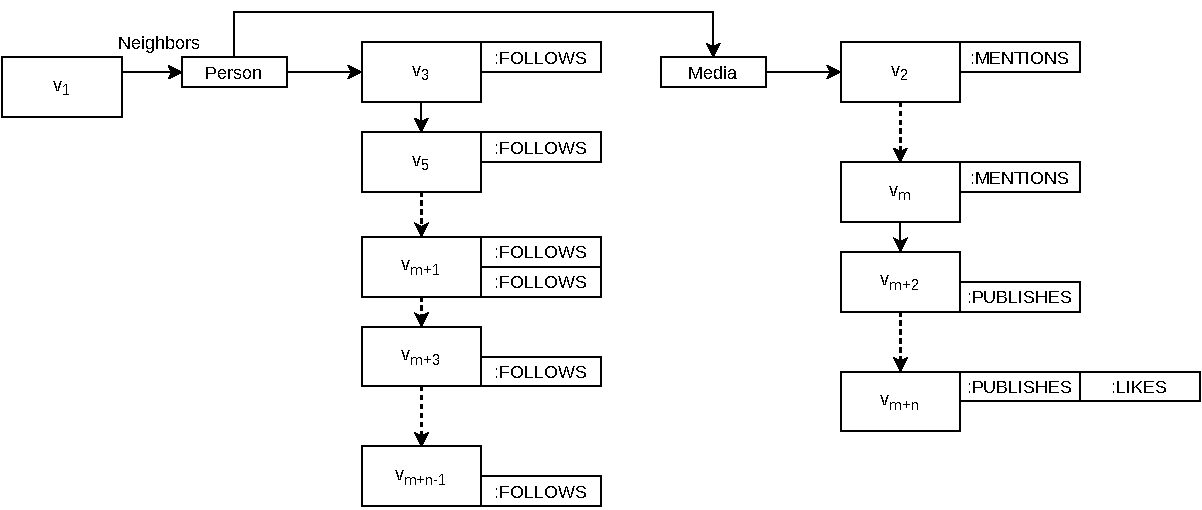
\includegraphics[width=0.48\textwidth]{img/data_neighbors.pdf}
%%   \caption{The vertex-centric storage structure of the celebrity $v_1$ in Figure~\ref{img:celebrity_star}.}\label{img:data_neighbors}
%% \end{figure}

From a higher perspective, in order to solve a property graph matching problem,
one need to firstly select a root vertex in the data graph.
%% regardless of the concrete graph matching algorithm whether it is tree based or join based.
There is no need to scan all the vertices in a billion node data graph if we only care about vertices with the specific labels.
Just like the local index we discussed above, we could add a global index which contains key-value pairs that maps the labels to the corresponding position on disk (Figure~\ref{img:data_example}).

The super-linear index problem of existing work was pointed out by~\cite{DBLP:journals/pvldb/SunWWSL12},
where indexes grow \emph{super-linearly} with respect to the \emph{edges}.
In contrast, indexes of SeqStar grows \emph{linearly} with respect to the \emph{vertices}.
In SeqStar, the length of global index is the length of vertex labels ($l$),
and the size of local indexes is bound to $l \times n$ ($n$ is the length of vertices).
%% In summery, for a property graph matching problem, we could quickly jump to the domain of interest with the help of the global index, and then scan and check only the necessary neighbors with the help of our local index.
%% After jump to the correct position, all the disk reads are sequential.
%% \begin{figure}[ht]
%%   \centering
%%   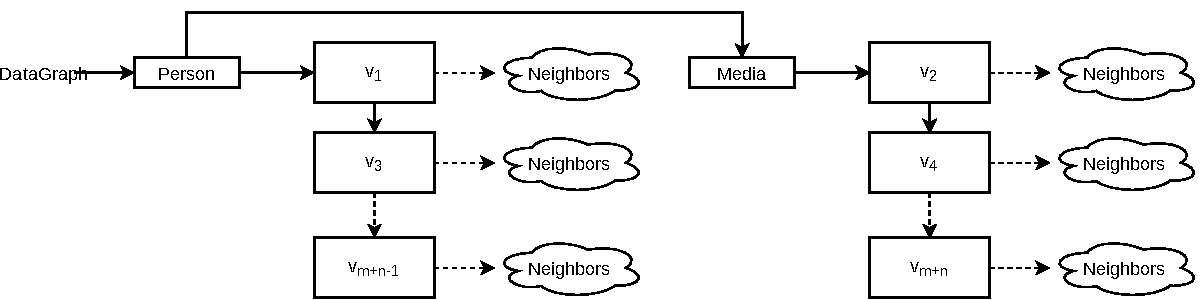
\includegraphics[width=0.48\textwidth]{img/data_vertices.pdf}
%%   \caption{The storage structure overview of the data graph in Figure~\ref{img:celebrity_star}.}\label{img:data_vertices}
%% \end{figure}
\subsection{Remarks on the Implementation of the Storage Method}\label{sec:storage_iterators}
For applications that need to perform the two basic operations (visiting vertices and visiting the neighbors),
we define two iterators as the interface to visit the data graph:
\begin{enumerate}[noitemsep]
\item \textsc{VertexIter}: Given a vertex label, it iterates through the vertices with the specified label ordered by the ID of vertices;
\item \textsc{NeighborIter}: Given a data vertex and a label, it visits the neighbors with the label, the neighbors are also sorted by the IDs.
\end{enumerate}
%% In Section~\ref{sec:match} we'll show that the sorting constraint could boost the matching of property graphs.

These iterators could be implemented efficiently by using SeqStar's vertex-centric storage model.
And we also provide a compact disk format implementing the vertex-centric storage model in Figure~\ref{img:data_graph}.
Vertices are sorted by their IDs, and we store in/out-degrees as early filters when scanning the vertices.
Edge labels are stored as integers here, however, bitmap could also be used for higher performance.
The \textsc{VertexIter} just searches the global index and then visits the disk data sequentially;
The \textsc{NeighborIter} scans the neighbors with the help of the local index.

Note that the vertex-centric storage model is not restricted to this disk format.
In fact, as long as a storage engine could implement the two iterators efficiently,
it could implement the vertex-centric storage model well.
For example, the sorted vertices could be replaced with B-tree to make the insertion/deletion operation easier for dynamic graphs.
%% It is also possible to implement the vertex-centric storage model in memory as buffer cache for existing graph databases to achieve better locality.
Moreover, we are now working on implementing the vertex-centric storage model on top of relational database to embrace the power of the half-century-year-old mature technology.
\begin{figure}[ht]
  \centering
  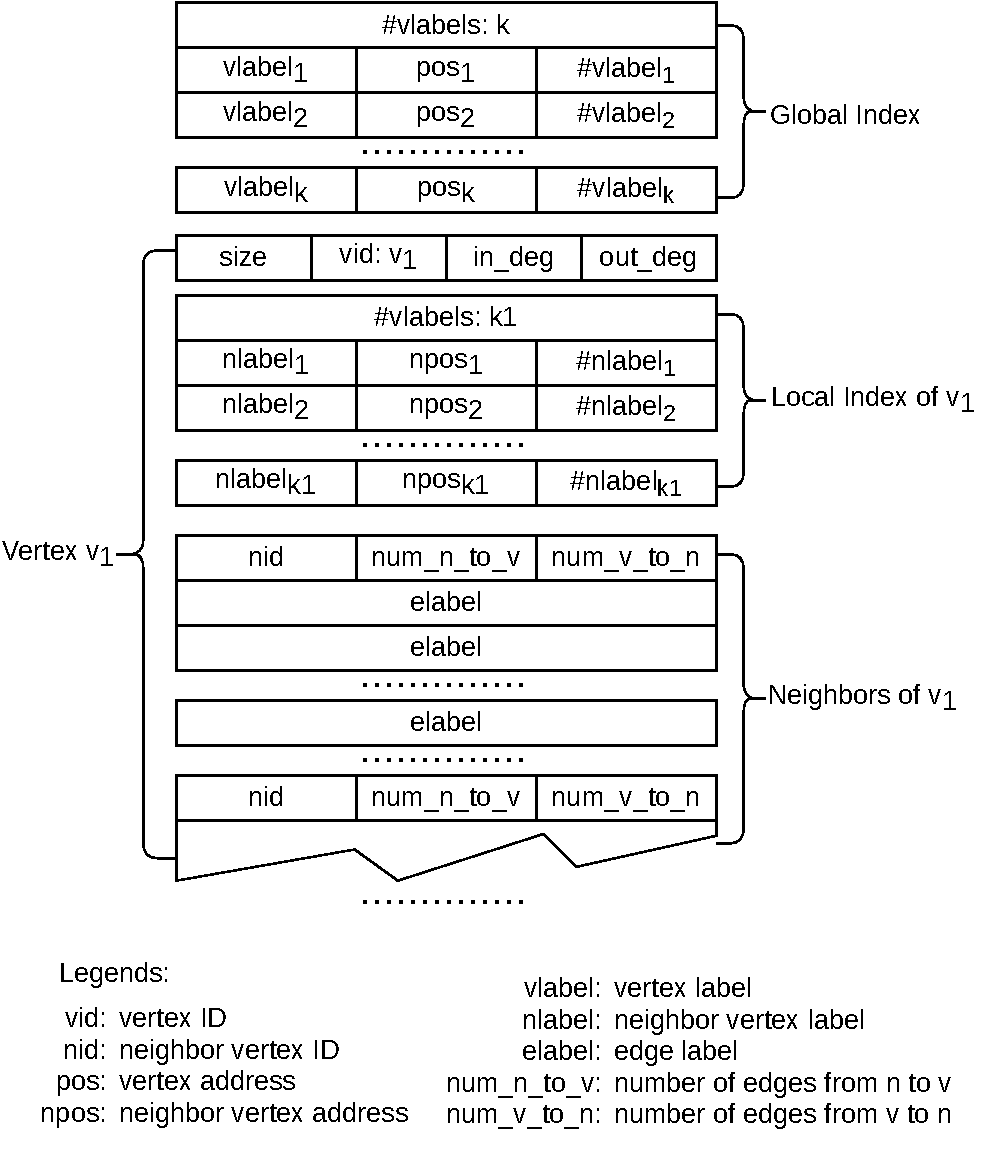
\includegraphics[width=0.48\textwidth]{img/data_graph.pdf}
  \caption{An I/O efficient property graph storage method that can boost the graph matching process.}\label{img:data_graph}
\end{figure}
